\begin{defn}
    The \textit{Dirichlet function }on $[0,1]$ is 
    \begin{equation}
        \label{Equ:Diri_Func}
        D(x)=\left\{
            \begin{array}{rl}
                1&x\in \mathbb{Q},\\
                0&x\notin\mathbb{Q}.
            \end{array}
        \right.
    \end{equation}
\end{defn}
\begin{exc}
    Show \eqref{Equ:Diri_Func} isn't Riemann integrable on $[0,1]$.
\end{exc}
\begin{proof}
    If $\Delta$ is a partition on $[0,1]$,
    \begin{displaymath}
        \Delta:0<x_1<x_2<\ldots<x_n=1,
    \end{displaymath}
    Set $\xi=(\xi_n)$, where $\xi_k\in[x_{k-1},x_k]$ is rational number,
    then $S(\Delta,\xi)=\sum_{k=1}^{n}D(\xi_k)\Delta x_K=1$.
    However, if set $\eta=(\eta_n)$, where $\eta_k\in[x_{k-1},x_k]$
    is irrational number, 
    then $S(\Delta,\eta)=\sum_{k=1}^{n}D(\eta_k)\Delta x_K=0$, 
    which means $\lim_{||\Delta||\rightarrow 0}S(\Delta,\xi)=1$,
    but $\lim_{||\Delta||\rightarrow 0}S(\Delta,\eta)=0$. 
    $D(x)$ is not Riemann integrable on $[0,1]$.
\end{proof}
\begin{rem}
    $D(x)=0$ a.e. on $[0,1]$, so we expact $\int_{0}^{1}D(x)\dif x=0$, 
    but $D(x)$ isn't Riemann integrable. 
    In this chapter, we introduce \textit{Lebesgue integral} to 
    handle this problem.
\end{rem}
\section{Measurable Functions}
\begin{defn}
    \label{Def:Preimage}
    Given a function $f:X\rightarrow Y$, $E\subset Y$, 
    \begin{displaymath}
        f^{-1}(E):=\{x\in X:f(x)\in E\}
    \end{displaymath}
    is the \textit{preimage} of $E$ related to $f$.
\end{defn}
\begin{prop}
    \label{Prop:PreimageProp}
    \begin{enumerate}
        \item $f^{-1}(\cup_{\lambda}E_{\lambda})
        =\cup_{\lambda}f^{-1}(E_{\lambda})$. 
        \item $f^{-1}(\cap_{\lambda}E_{\lambda})
        =\cap_{\lambda}f^{-1}(E_{\lambda})$.
        \item $f^{-1}(E^c)=(f^{-1}(E))^{c}$.
        \item If $\mathcal{N}$ is a $\sigma$-algebra on $Y$, 
        then $\{f^{-1}(E):E\in\mathcal{N}\}$ is a 
        $\sigma$-algebra on $X$.
    \end{enumerate}
\end{prop}
\begin{exc}
    Prove Proposition \ref{Prop:PreimageProp}.
\end{exc}
\begin{proof}
    For the first rule, $\forall x\in f^{-1}(\cup_{\lambda}E_{\lambda})$,
    $f(x)\in\cup_{\lambda}E_{\lambda}$, so $\exists \lambda_x$, s.t.
    $f(x)\in E_{\lambda_x}$, which means $x\in f^{-1}(E_{\lambda_x})$,
    so $x\in \cup_{\lambda}f^{-1}(E_{\lambda})$. On the other hand,
    $\forall y\in\cup_{\lambda}f^{-1}(E_{\lambda})$, 
    $\exists \lambda_y$, s.t. $y\in f^{-1}(E_{\lambda_y})$,
    so $y\in f^{-1}(\cup_{\lambda}E_{\lambda})$. 
    Thus, it's easy to conclude that  
    $f^{-1}(\cup_{\lambda}E_{\lambda})
    =\cup_{\lambda}f^{-1}(E_{\lambda})$.

    The second rule can be proved in the same way as the first one.

    As for the third one, $\forall x\in f^{-1}(E^c)$, so $f(x)\notin E$,
    which means $x\in(f^{-1}(E))^{c}$. On the other hand,
    $\forall y\in(f^{-1}(E))^{c}$, so $y\notin f^{-1}(E)$,
    which means $f(y)\in E^c$, so $y\in f^{-1}(E^c)$.
    Thus, it's easy to conclude that $f^{-1}(E^c)=(f^{-1}(E))^{c}$.

    The fourth rule can be easily proved by the first three rules
    and the Definition \ref{Defn:SigmaAlg}.
\end{proof}
\begin{defn}
    \label{Def:MeasurableFunc}
    If $(X,\M)$, $(Y,\mathcal{N})$ are measurable spaces, 
    $f:X\rightarrow Y$ is called \textit{$(\M,\mathcal{N})$-measurable} 
    if $\forall E\in\mathcal{N}$, $f^{-1}(E)\in\M$.
\end{defn}
\begin{prop}
    \label{Prop:DescribeMeasFunc}
    If $\mathcal{N}=\M(\mathcal{E})$, then $f:X\rightarrow Y$ is 
    measurable iff $\forall E\in\mathcal{E}$, $f^{-1}(E)\in\M$.
\end{prop}
\begin{proof}
    $"\Rightarrow"$: Follows directly by Definition 
    \ref{Def:MeasurableFunc}.
    
    $"\Leftarrow"$: By Proposition \ref{Prop:PreimageProp}, 
    $\mathcal{A}:=\{E\subset Y:f^{-1}(E)\in\M\}$ is a $\sigma$-algebra, 
    and by the condition, this $\sigma$-algebra contains $\mathcal{E}$, 
    so $\mathcal{A}\supset\mathcal{M}(\mathcal{E})=\mathcal{N}$, 
    i.e. $f$ is a measurable function.  
\end{proof}
\begin{coro}
    \label{Cor:ContinuousMeas}
    If $(X,\tau_1)$, $(Y,\tau_2)$ are topological spaces and 
    $f:X\rightarrow Y$ is continuous, then 
    $f$ is $(\mathcal{B}_{X},\mathcal{B}_{Y})$-measurable.
\end{coro}
\begin{exc}
    Prove Corollary \ref{Cor:ContinuousMeas}.
\end{exc}
\begin{proof}
    $f:X\rightarrow Y$ is continuous $\Leftrightarrow$ 
    $\forall U\in\tau_2$, $f^{-1}(U)\in\tau_1$.
    By Definition \ref{Def:MeasurableFunc}, we know
    $f$ is $(\mathcal{B}_{X},\mathcal{B}_{Y})$-measurable.
\end{proof}
\begin{defn}
    \label{Defn:Mmeasurable}
    Given $(X,\M)$ be a measurable space, $f:X\rightarrow\mathbb{R}$ 
    (or $\mathbb{C}$) 
    is called \textit{$\M-$measurable} if $f$ is 
    $(\M,\mathcal{B}_{\mathbb{R}})$ (or $(\M,\mathcal{B}_{\mathbb{C}})$) 
    measurable.
\end{defn}
\begin{defn}
    $f:\mathbb{R}\rightarrow\mathbb{C}$ is \textit{Lebesgue Measurable} 
    if it is $(\mathcal{L},\mathcal{B}_{\mathbb{C}})$-measurable, 
    $f$ is Borel measurable if it is 
    $(\mathcal{B}_{\mathbb{R}},\mathcal{B}_{\mathbb{C}})$-measurable.
\end{defn}
\begin{exc}
    \label{Exc:ComposeOfMeasurable}
    Assume $f,g:\mathbb{R}\rightarrow\mathbb{R}$, 
    If $f$ is Borel measurable and $g$ is Lebesgue measurable, 
    then $f\circ g$ is Lebesgue measurable.
\end{exc}
\begin{proof}
    $\forall E\in\mathcal{B}_{\mathbb{R}}$,by $f$ is Borel measurable,
    so $f^{-1}(E)\in\mathcal{B}_{\mathbb{R}}$, and by 
    $g$ is Lebesgue measurable, $(f\circ g)^{-1}(E)=
    g^{-1}(f^{-1}(E))\in\mathcal{L}$, then $f\circ g$ is Lebesgue measurable.
\end{proof}
\begin{defn}
    \label{Defn:CantorFunc}
    If $\mathcal{C}$ is the \textit{Cantor set} on $[0,1]$
    (see Definition \ref{Defn:CantorSet}), 
    the \textit{Cantor function} $c:[0,1]\rightarrow[0,1]$ 
    is:
    \begin{equation}
        \label{Equ:CantorFunc}
        c(x)=\left\{
            \begin{array}{rl}
                \sm{n}{\infty}\frac{a_n}{2^{n}},&
                x=\sm{n}{\infty}\frac{2a_n}{3^n}\in\mathcal{C}
                ;\\
                \sup_{y\le x,y\in\mathcal{C}}c(y),&x\in[0,1]\setminus
                \mathcal{C}.\\
            \end{array}
        \right.
    \end{equation}
    \begin{figure}[H]
        \centering
        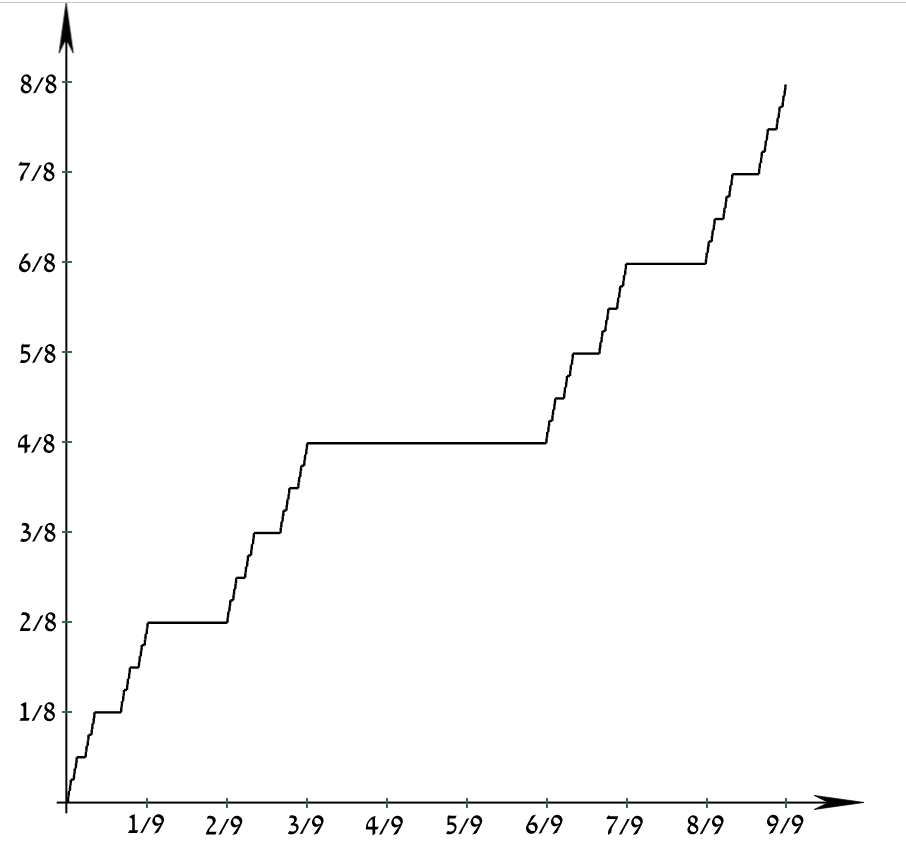
\includegraphics
        [width=\linewidth,height=0.2\textheight]{png/CantorFunc.png}
        \caption{Cantor function, download from Wikipedia.}
    \end{figure}
\end{defn}
\begin{exc}
    Let $f:[0,1]\rightarrow[0,1]$ be the Cantor function, 
    and let $g(x)=f(x)+x$.
    \begin{enumerate}
        \item $g$ is a bijection from $[0,1]$ to $[0,2]$, 
        and $h=g^{-1}$ is continuous from $[0,2]$ to $[0,1]$.
        \item If $C$ is a Cantor set, $m(g(C))=1$.
        \item $g(C)$ contains a Lebesgue nonmeasurable set $A$. 
        Let $B=g^{-1}(A)$, $B$ is Lebesgue measurable but not Borel.
        \item There exist a Lebesgue measurable function $F$ and a 
        continuous function $G$ on $\mathbb{R}$ such that 
        $F\circ G$ is not Lebesgue measurable.
    \end{enumerate}
\end{exc}
\begin{proof}
    (1)$f(x)$ is monotone increasing, and naturally $p(x)=x$
    is a strictly increasing function, and hence $g(x)=f(x)+x$
    x is also strictly increasing and therefore injective. 
    Next, to show surjectivity, note that $g$ is a continuous function, 
    and $g(0)=0$, $g(1)=2$; hence, by the intermediate value theorem, 
    $g$ is surjective. We now have all the necessary components to 
    conclude that $g$ is a bijection, and since $g$ is a
    continuous bijective function, and $[0,1]$ is compact, 
    $g^{-1}$ is continuous from $[0,2]$ to $[0,1]$.

    (2)Firstly, by $g$'s surjectivity, and $C$ being measurable, 
    we see that:
    \begin{displaymath}
        \begin{array}{rl}
            g([0,1]\setminus C)\cup g(C)=g([0,1]\cap C^c)\cup g(C)=[0,2]\\
            \Rightarrow m(g(C))+m(g([0,1]\setminus C))=2.
        \end{array}
    \end{displaymath}
    Next, since $C$ is a closed set $\Rightarrow$ $[0,1]\setminus C$
    is open set. Therefore, since all open subsets of $[0,1]$ may
    be written as a countable union of disjoint open sets, 
    let us write $[0,1]\setminus C=\cup_{1}^{\infty}O_j$, $O_j=(a_j,b_j)$.
    Now, since $f$ is by construction constant on $[0,1]\setminus C$,
    and $m(C)=0\Rightarrow m([0,1]\setminus C)=1\Rightarrow
    m(\cup_{1}^{\infty}O_j)=1$.
    \begin{displaymath}
        \begin{array}{rl}
            m(g([0,1]\setminus C))&=m(g(\cup_{1}^{\infty}O_j))
            =\sum_{1}^{\infty}m(g(O_j))\\
            &=\sum_{1}^{\infty}(m(f(b_j)-f(a_j))+m(b_j-a_j))\\
            &=\sum_{1}^{\infty}m(O_j)\\
            &=m(\cup_{1}^{\infty}O_j)\\
            &=1
        \end{array}
    \end{displaymath}  
    And hence $m(g(C))=1$.
    
    (3)To show Lebesgue measurability, naturally $B\subset C$,
    and since $C$ is measurable with measure $m(C)=0$, it implies
    $m(B)\leq m(C)=0$, and hence Lebesgue measurable since null 
    sets are measurable. For the sake of contradiction, suppose
    $B=g^{-1}(A)$ is Borel measurable. In part (1), we showed that
    $g^{-1}$ is continuous and bijective; therefore 
    $g(B)=g(g^{-1}(A))=A$. However, by the continuity of $g$,
    if $g^{-1}(A)$ was Borel, so too would $g(g^{-1}(A))=A$,
    hence a contradiction since $A$ is not Lebesgue
    measurable; therefore, $B$ cannot be Borel measurable.

    (4)Let $F=\chi_{B}$;
    \begin{equation}
        F(x)=\left\{
            \begin{array}{rl}
                1, &x\in B, \\
                0, &x\notin B,
            \end{array}
        \right.
    \end{equation}
    And also set $G=g^{-1}$. Naturally $G$ is Lebesgue measurable 
    since it is continuous, we now wish to prove that so too is $F$. 
    This can be seen by noticing $F^{-1}((a,\infty))=\emptyset$ or $B$
    or $\mathbb{R}$, , but all these possibilities are Lebesgue measurable,
    hence $F$ is Lebesgue measurable. We can now look at the following 
    reasoning:
    \begin{displaymath}
        \begin{array}{rl}
            (F\circ G)^{-1}([\frac{1}{2},\infty))&=G^{-1}\circ F^{-1}([\frac{1}{2},\infty))\\
            &=\{x\in[0,2]|\chi_B(g^{-1}(x))\in[\frac{1}{2},\infty)\} \\
            &=\{x\in[0,2]|g^{-1}(x)\in B\} \\
            &=G^{-1}(B)=g(g^{-1}(B))=A,
        \end{array}
    \end{displaymath}
    Now since $A$ is not Lebesgue measurable, 
    $F\circ G$ also will not be Lebesgue measurable.
\end{proof}
\begin{prop}
    \label{Prop:ComplexMeasurableFunc}
    $f:X\rightarrow\mathbb{C}$ is $\M$-measurable iff $\text{Re}f$, 
    $\text{Im}f$ are $\M$-measurable. 
\end{prop}
\begin{proof}
    Choose $\pi_{1}(z):=\text{Re}z$, $\pi_{2}(z):=\text{Im}z$, 
    then $\pi_{1},\pi_{2}$ are both measurable. If $f$ is 
    $\M$-measurable, 
    then $\text{Re}f=\pi_{1}\circ f$, $\text{Im}f=\pi_{2}\circ f$ 
    are both $\M$-measurable.

    If $\text{Im}f$, $\text{Re}f$ are both measurable, i.e. 
    $\pi_1\circ f$, $\pi_{2}\circ f$ are measurable, then for 
    any Borel set $\mathcal{B}\subset\mathbb{R}$, 
    $f^{-1}(\pi_{\alpha}^{-1}(\mathcal{B}))\in\M$ for 
    $\alpha=1,2$. $f$ is measurable 
    follows from $\mathcal{B}_{\mathbb{C}}
    =\mathcal{B}_{\mathbb{R}}\otimes
    \mathcal{B}_{\mathbb{R}}$ and 
    Proposition \ref{Prop:DescribeMeasFunc}.
\end{proof}
\begin{prop}
    \label{Prop:MeasFuncLinear}
    If $f,g:X\rightarrow\mathbb{C}$ are 
    $\M$-measurable, so are $f+g$, $fg$. 
\end{prop}
\begin{proof}
    Define $F:X\rightarrow \mathbb{C}\times\mathbb{C}$, 
    $F(x):=(f(x),g(x))$, 
    $\phi,\psi:\mathbb{C}\times\mathbb{C}\rightarrow\mathbb{C}$ 
    are 
    \begin{displaymath}
        \phi(z,w):=z+w,\quad \psi(z,w):=zw,
    \end{displaymath}
    then $F$ is 
    $(\M,\mathcal{B}_{\mathbb{C}\times\mathbb{C}})$-measurable, 
    $\phi,\psi$ are 
    $(\mathcal{B}_{\mathbb{C}\times\mathbb{C}},
    \mathcal{B}_{\mathbb{C}})$-measurable. So are 
    $f+g=\phi\circ F$, $fg=\psi\circ F$.
\end{proof}
\begin{rem}
    Proposition \ref{Prop:MeasFuncLinear} shows that 
    all the $\M$-measurable functions form an algebra.
\end{rem}
\begin{ntn}
    The \textit{generalized real line} 
    is denoted by:
    \begin{displaymath}
        \bar{\mathbb{R}}:=[-\infty,\infty]
        =\mathbb{R}\cup\{-\infty,\infty\}.
    \end{displaymath}
\end{ntn}
\begin{prop}
    \label{Prop:LimitProperties}
    $\forall j\in\mathbb{N}$, 
    $f_{j}:X\rightarrow\bar{\mathbb{R}}$ are 
    measurable functions, then 
    $g_{1}(x):=\limsup_{j\rightarrow\infty}f_{j}(x)$, 
    $g_{2}(x):=\liminf_{j\rightarrow\infty}f_{j}(x)$ 
    are measurable.
\end{prop}
\begin{exc}
    Prove Proposition \ref{Prop:LimitProperties}.
\end{exc}
\begin{proof}
    Set $m(x)=\sup_{j}f_{j}(x)$, $n(x)=\inf_{j}f_{j}(x)$.
    By the truth that $f_{j}:X\rightarrow\bar{\mathbb{R}}$ are 
    measurable functions, $m^{-1}((a,\infty])=
    \cup_{1}^{\infty}f_{j}^{-1}((a,\infty])$,  $n^{-1}([\infty,a))=
    \cup_{1}^{\infty}f_{j}^{-1}([\infty,a))$, so $m(x)$, $n(x)$
    are measurable. More generally, if $h_k(x)=\sup_{j>k}f_j(x)$
    then $h_k$ is measurable for each $k$, so $g_1(x)=\inf_{k}h_k(x)$
    is measurable, and likewise for $g_2(x)$.
\end{proof}
\begin{defn}
    Given $f:X\rightarrow\bar{\mathbb{R}}$, 
    the \textit{positive part }of $f$ is:
    \begin{displaymath}
        f^{+}(x):=\max(f(x),0),
    \end{displaymath}
    and the \textit{negative part }of $f$ 
    is:
    \begin{displaymath}
        f^{-}(x):=\max(-f(x),0).
    \end{displaymath}
\end{defn}
\begin{rem}
    If $f$ is measurable, so are $f^{+}$ and 
    $f^{-}$.
\end{rem}
\begin{defn}
    Given $f:X\rightarrow\mathbb{C}$, the 
    \textit{polar decomposition }of $f$ is 
    $f:=(\sgn f)|f|$ where 
    \begin{displaymath}
        \sgn(z)=\left\{
            \begin{array}{rl}
                \frac{z}{|z|},z\neq 0;
                0,z=0.
            \end{array}
        \right.
    \end{displaymath}
\end{defn}
\begin{rem}
    If $f$ is measurable, so are $\sgn f$ and $|f|$.
\end{rem}
\begin{defn}
    \label{Defn:CharFunc}
    For $E\subset X$, the \textit{characteristic function} of $X$ 
    is given by $\chi_{E}(x)$ with:
    \begin{displaymath}
        \chi_{E}(x):=\left\{
            \begin{array}{rl}
                1,x\in E;\\
                0,x\notin E.\\
            \end{array}
        \right.
    \end{displaymath}
\end{defn}
\begin{defn}
    \label{Defn:SimpleFunc}
    A \textit{simple function }on $X$ is given by 
    $f:X\rightarrow\mathbb{C}$ with 
    $f(x)=\sm{j}{n}z_{j}\chi_{E_{j}}$, where $E_j\in\M$, 
    $z_j\in\mathbb{C}$, satisfies $\forall j\neq k$ $z_{j}\neq z_{k}$, 
    $E_j\cap E_k=\emptyset$.
\end{defn}
\begin{thm}
    \label{Thm:ApproxMeasFuncBySimpleFunc}
    If $f:X\rightarrow[0,\infty]$ is measurable, 
    then there exists simple functions $\{\phi_{n}\}$ such that 
    $0\le\phi_{1}\le\ldots\le\phi_{n}\le\ldots\le f$, 
    $\phi_{n}\rightarrow f$ pointwise, and 
    $\phi_{n}\rightarrow f$ uniformly in any set 
    where $f$ is bounded.
\end{thm}
\begin{exc}
    For $0\le k\le 2^{2n}-1$, mark 
    \begin{displaymath}
    E_{n}^{k}:=f^{-1}((k2^{-n},(k+1)2^{-n}]),\quad 
    F_{n}:=f^{-1}((2^{n},\infty]),
    \end{displaymath}
    then define 
    \begin{displaymath}
        \phi_{n}:=\sum_{k=0}^{2^{2n}-1}k2^{-n}\chi_{E_{n}^{k}}
        +2^{n}\chi_{F_{n}},
    \end{displaymath}
    show $\{\phi_{n}\}$ satisfies the condition of 
    Theorem \ref{Thm:ApproxMeasFuncBySimpleFunc}.
\end{exc}
\begin{proof}
    By the truth that $\chi_{E}(x)\geq 0$, it is easily checked
    that $\phi_{n}\leq\phi_{n+1}$ for all $n$, and 
    $0\leq f-\phi_{n}\leq 2^{-n}$ on the set where 
    $f\leq 2^{-n}$. The result therefore follows.
\end{proof}
\section{Integration}
\begin{defn}
    \label{Defn:IntegralOfSimpleFunc}
    Given a measurable space $(X,\M,\mu)$, define 
    \begin{displaymath}
        \mathcal{L}^{+}:=\{\text{measurable functions }f:
        X\rightarrow[0,\infty]\},
    \end{displaymath}
    if $\phi\in \mathcal{L}^{+}$ is a simple function with 
    $\phi=\sm{i}{n}\phi_{i}\chi_{E_i}$, then 
    the \textit{integration of $\phi$} is 
    \begin{displaymath}
        \int\phi\dif\mu:=\sm{i}{n}\phi_{i}\mu(E_i).
    \end{displaymath}
\end{defn}
\begin{rem}
    We mark $0\cdot\infty=0$.
\end{rem}
\begin{prop}
    \label{Prop:PropertyOfSimpleInt}
    For simple functions $\phi$, $\psi\in\mathcal{L}^{+}$. 
    \begin{enumerate}
        \item If $c\ge 0$, then $\int c\phi=c\int\phi$. 
        \item $\int(\phi+\psi)=\int\phi+\int\psi$.
        \item If $\phi\le\psi$, then $\int\phi\le\int\psi$. 
        \item $A\mapsto \int_{A}\phi\dif\mu$ is a measure on $\M$.
    \end{enumerate}
\end{prop}
\begin{exc}
    Prove Proposition \ref{Prop:PropertyOfSimpleInt}.
\end{exc}
\begin{proof}
    (a) id trivial. For (b), let $\sum_{1}^{n}a_j\chi_{E_j}$ and 
    $\sum_{1}^{m}b_k\chi_{F_k}$ be the standard representation of 
    $\phi$ and $\psi$. Then $E_j=\cup_{k=1}^{m}(E_j\cap F_k)$ and
    $F_k=\cup_{j=1}^{n}(E_j\cap F_k)$ since $\cup_{1}^{n}E_j=
    \cup_{1}^{m}F_k=X$, and these unions are disjoint. Hence the
    finite additivity of $\mu$ implies that
    \begin{displaymath}
        \int\phi+\int\psi=\sum_{j,k}(a_j+b_k)\mu(E_j\cap F_k),
    \end{displaymath}
    and the same reasoning show that the sum on the right equals
    $\int(\phi+\psi)$. Moreover, if $\phi\leq\psi$, then $a_j\leq b_k$
    whenever $E_j\cap F_k\neq\emptyset$, so
    \begin{displaymath}
        \int\phi=\sum_{j,k}a_j\mu(E_j\cap F_k)\leq\sum_{j,k}b_k\mu(E_j\cap F_k)
        =\int\psi,
    \end{displaymath}
    which proves (c). Finally, if $\{A_k\}$ is a disjoint sequence in $\mathcal{M}$
    and $A=\cup_{1}^{\infty}A_k$,
    \begin{displaymath}
        \int_A\phi=\sum_ja_j\mu(A\cap E_j)=\sum_{j,k}a_j\mu(A_k\cap E_j)
        =\sum_k\int_{A_k}\phi,
    \end{displaymath}
    which establishes (d).
\end{proof}
\begin{defn}
    \label{Defn:IntegralForPositive}
    For $f\in \mathcal{L}^{+}$, define 
    \begin{displaymath}
        \int f\dif\mu:=\sup\left\{\int\phi\dif\mu:0\le\phi\le f,
        \;\phi\text{ is simple}\right\}.
    \end{displaymath}
\end{defn}
\begin{rem}
    Definition \ref{Defn:IntegralForPositive} is straightforward 
    from Theorem \ref{Thm:ApproxMeasFuncBySimpleFunc}.
\end{rem}
\begin{defn}
    \label{Defn:RealValuedFuncInt}
    If $f:X\rightarrow\bar{\mathbb{R}}$, we say 
    $f$ is \textit{integrable} iff $\int|f|\dif\mu<\infty$, 
    then 
    \begin{displaymath}
        \int f\dif\mu:=\int f^{+}\dif\mu-\int f^{-}\dif\mu.
    \end{displaymath}
\end{defn}
\begin{defn}
    \label{Defn:ComplexValuedFuncInt}
    If $f:X\rightarrow\mathbb{C}$, we say $f$ is \textit{integrable} 
    iff $\int|f|\dif\mu<\infty$, then 
    \begin{displaymath}
        \int f\dif\mu=\int \text{Re}f\dif\mu+i\int\text{Im}f\dif\mu.
    \end{displaymath}
\end{defn}
\begin{exc}
    Show that all the integrable 
    functions on $X$ forms a vector space.
\end{exc}
\begin{proof}
    We only need to prove that all the integrable 
    functions on $X$ satisfy their closure under addition
    and their closure under scalar multiplication. 
    $\forall \lambda\in\mathbb{C}$ and if $f$ 
    is \textit{integrable}, then 
    $\int|\lambda f|d\mu=|\lambda|\int|f|d\mu<\infty$,
    so $\lambda f$ is \textit{integrable}.
    If $f$ and $g$ is \textit{integrable},
    $\int|f+g|d\mu\leq\int|f|d\mu+\int|g|d\mu<\infty$,
    so $f+g$ is \textit{integrable}.
\end{proof}
\begin{ntn}
    If the measure $\mu$ is clear, 
    we write $\int\phi$ to 
\end{ntn}
\begin{thm}[Monotone Convergence Theorem]
    \label{Thm:MCT}
    If $\{f_{n}\}\subset\mathcal{L}^{+}$ such that 
    $\forall j\in\mathbb{N}$, $f_j\le f_{j+1}$, and 
    $f=\lim_{n\rightarrow\infty}f_{n}$, then 
    $\int f=\lim_{n\rightarrow\infty}\int f_n$.
\end{thm}
\begin{proof}
    We divide this proof into 3 steps. 

    First, since $\forall x\in X$, $\{f_{n}(x)\}$ is an increasing 
    sequence on $[0,\infty]$, $f(x):=\lim_{n\rightarrow\infty}f_{n}(x)$ 
    exists in $[0,\infty]$ as well, and $\forall n\in\mathbb{N}$, 
    $f_{n}(x)\le f(x)$.

    Second, $\forall n\in\mathbb{N}$, $f_{n}\le f$ means 
    \begin{displaymath}
        \forall n\in\mathbb{N}, \int f_{n}\le\int f,
    \end{displaymath}
    choose $n\rightarrow\infty$, 
    it shows $\lim_{n\rightarrow\infty}f_{n}\le\int f$.

    Third, given $\alpha\in(0,1)$ and simple function $\phi$ 
    such that $0\le\phi\le f$, let 
    \begin{displaymath}
        E_n:=\{x:f_{n}(x)\ge\alpha\phi(x)\},
    \end{displaymath}
    then $E_{n}$ is increasing, and $\cp{n}{\infty}E_n=X$, thus:
    \begin{displaymath}
        \forall\alpha\in(0,1),\;
        \int f_n\ge\int_{E_n}f_{n}\ge\alpha\int_{E_n}\phi.
    \end{displaymath}
    Set $n\rightarrow\infty$, it yields $\forall\alpha\in(0,1)$, 
    \begin{displaymath}
        \lim_{n\rightarrow\infty}\int f_n\ge\alpha\int\phi.
    \end{displaymath}
    So $\lim_{n\rightarrow\infty}\int f_n\ge\int\phi$. 
    Choose supermum, it means 
    $\lim_{n\rightarrow\infty}f_n\ge\int f$. 
    It completes the proof.
\end{proof}
\begin{exc}
    In the proof of Theorem \ref{Thm:MCT}, 
    can we replace $\alpha\phi$ by $\phi-\epsilon$? 
    Why?
\end{exc}
\begin{proof}
    No! It may make $\phi-\epsilon\leq0$ in some measurable
    sets $E_j$.
\end{proof}
\begin{thm}
    \label{Thm:SeriesAndInt}
    For $\{f_n\}\subset \mathcal{L}^{+}$, 
    $f:=\sm{n}{\infty}f_n$, 
    $\int f=\sm{n}{\infty}\int f_n$.
\end{thm}
\begin{exc}
    Prove Theorem \ref{Thm:SeriesAndInt}.
\end{exc}
\begin{proof}
    Let $\phi_n=\sum_{1}^{n}f_n$, since 
    $\{f_n\}\subset\mathcal{L}^{+}$, 
    $\{\phi\}\subset\mathcal{L}^{+}$, such that 
    $\forall j\in\mathbb{N}$, $\phi_j\leq\phi_{j+1}$, and
    $f=\lim_{n\rightarrow\infty}\phi_n$,
    then by Theorem \ref{Thm:MCT} $\int f=\lim_{n\rightarrow\infty}\int\phi_n
    =\lim_{n\rightarrow\infty}\int\sum_{1}^{n}f_n
    =\sum_{1}^{\infty}\int f_n$.
\end{proof}
\begin{rem}
    Theorem \ref{Thm:SeriesAndInt} shows that 
    term-by-term integration property holds 
    for positive functions.
\end{rem}
\begin{prop}
    \label{Prop:PositiveIntZero}
    If $f\in \mathcal{L}^{+}$, then 
    $\int f=0\Leftrightarrow f=0$ a.e..
\end{prop}
\begin{proof}
    We divide this proof into three steps. 

    First, if $f$ is a simple function, i.e. 
    $f=\sm{i}{n}a_{i}\chi_{E_i}$, then 
    \begin{displaymath}
        \int f=0\Leftrightarrow
        \sm{i}{n}a_{i}\mu(E_i)=0.
    \end{displaymath}
    Since $a_{i}\ge 0$, if $a_{i_{0}}>0$, 
    it means 
    \begin{displaymath}
        \sm{i}{n}a_{i}\mu(E_i)
        \ge a_{i_0}\mu(E_{i_0})=0,
    \end{displaymath}
    i.e. $\mu(E_{i_0})=0$, it means $f=0$ a.e..
    If for a simple function $f$, $f=0$ a.e., it's clear that 
    $\int f=0$.

    Second, for $f\in \mathcal{L}^{+}$, if $f=0$ a.e., 
    $\forall$ simple function $0\le\phi\le f$, 
    $\phi=0$ a.e., so $\int\phi=0$, which means $\int f=0$.

    Finally, if $\int f=0$, let $E_{n}:=\{x:f(x)>\frac{1}{n}\}$, 
    then $\cp{n}{\infty}E_{n}=\{x:f(x)\neq 0\}$. 
    Assume $f=0$ a.e. isn't true, it means $\exists E_{n}$ 
    such that $\mu(E_n)>0$. 
    But 
    \begin{displaymath}
        \int f\ge\int_{E_n}f\ge\frac{1}{n}\int_{E_n}1
        =\frac{1}{n}\mu(E_n)>0,
    \end{displaymath}
    contradict! So $f=0$ a.e..
\end{proof}
\begin{coro}
    For $\{f_{n}\}\subset\mathcal{L}^{+}$, 
    $f\in\mathcal{L}^{+}$, 
    assume for a.e. $x\in X$, $\{f_{n}(x)\}$ is increasing and 
    $\lim_{n\rightarrow\infty}f_{n}(x)=f(x)$, 
    then 
    \begin{displaymath}
        \int f=\lim_{n\rightarrow\infty}\int f_n.
    \end{displaymath}
\end{coro}
\begin{thm}[Fatou's Lemma]
    \label{Thm:Fatou}
    For $\{f_{n}\}\subset\mathcal{L}^{+}$, 
    \begin{displaymath}
        \int\liminf_{n\rightarrow\infty}f_n\le\liminf_{n\rightarrow\infty}
        \int f_n.
    \end{displaymath}
\end{thm}
\begin{proof}
    $\forall k\ge 1$, $j\ge k$, $\inf_{n\ge k}f_n\le f_{j}$, 
    thus 
    \begin{displaymath}
        \forall j\ge k,\;
        \int\inf_{n\ge k}f_n\le\int f_{j}.
    \end{displaymath} 
    So 
    \begin{displaymath}
        \int\inf_{n\ge k}f_n\le\inf_{j\ge k}\int f_{j}.
    \end{displaymath}
    Then, since $g_{k}:=\inf_{n\ge k}f_{n}$ is increasing, 
    by Theorem \ref{Thm:MCT}, 
    \begin{displaymath}
        \begin{array}{rl}
        \int\liminf_{n\rightarrow\infty}f_{n}
        &=\int\lim_{k\rightarrow\infty}\inf_{n\ge k}f_{n}\\
        &=\lim_{k\rightarrow\infty}\int\inf_{n\ge k}f_{n}\\
        &\le\lim_{k\rightarrow\infty}\inf_{n\ge k}\int f_{n}\\
        &=\liminf_{n\rightarrow\infty}\int f_{n}.
        \end{array}
    \end{displaymath}
\end{proof}
\begin{exc}
    Give a sequence $\{f_{n}\}\subset\mathcal{L}^{+}$, 
    such that 
    \begin{displaymath}
        \int\liminf_{n\rightarrow\infty}f_{n}<
        \liminf_{n\rightarrow\infty}\int f_{n}.
    \end{displaymath}
\end{exc}
\begin{proof}
    We can consider function
    \begin{displaymath}
        f_n(x)=
        \left\{\begin{array}{rl}
            &n \quad \textit{for} \quad x\in(0,\frac{1}{n}),\\
            &0 \quad \textit{otherwise}\\
        \end{array}
        \right.
    \end{displaymath}
    These sequences converge pointwise (respectively uniformly) 
    to the zero function (with integral equal to zero), 
    yet each sequence has an integral of one.
\end{proof}
\begin{prop}
    \label{Prop:PropOfL1}
    \begin{enumerate}
        \item $f$ is integrable on $X$ 
        means $\{x:f(x)\neq 0\}$ is $\sigma$-finite. 
        \item If $f,g$ are integrable, then TFAE:
        \begin{enumerate}
            \item $\forall E\in\M$, $\int_{E}f=\int_{E}g$.
            \item $\int|f-g|=0$.
            \item $f=g$ a.e..
        \end{enumerate}
    \end{enumerate}
\end{prop}
\begin{proof}
    (1). If $f\in\mathcal{L}^{+}$, 
    $\forall n\in\mathbb{N}^{+}$, since $f$ is integrable, 
    $\mu(\{x:f(x)>\frac{1}{n}\})<\infty$. So $\{f>0\}$ is $\sigma$-finite. 
    If $f\in L^{1}$, then 
    \begin{displaymath}
        \{x:f(x)\neq 0\}=\{\text{Re}f\neq 0\}\cup\{\text{Im}f\neq 0\}
    \end{displaymath}
    is $\sigma$-finite. It completes the proof. 

    (2). $(b)\Leftrightarrow (c)$: Follows from Proposition 
    \ref{Prop:PositiveIntZero}.

    $(b)\Rightarrow (a)$: Since $\int|f-g|=0$, 
    \begin{displaymath}
        \begin{array}{rl}
        \left|\int_{E}f-\int_{E}g\right|
        &=\left|\int\chi_{E}(f-g)\right|\\
        &\le\int\left|\chi_{E}(f-g)\right|\\
        &\le\int|f-g|=0.\\
        \end{array}
    \end{displaymath}
    So $\int_{E}f=\int_{E}g$. 

    $(a)\Rightarrow (c)$: If $\mu(\{f\neq g\})\neq 0$, 
    choose $u:=\text{Re}(f-g)$, $v:=\text{Im}(f-g)$, 
    one of $u^{\pm},v^{\pm}$ is nonzero on some $E$ such that $\mu(E)>0$. 
    WLOG, say $E=\{u^{+}>0\}$, then 
    \begin{displaymath}
        \text{Re}\left(\int_{E}f-\int_{E}g\right)=\int_{E}u^{+}>0,
    \end{displaymath}
    contradict!
\end{proof}
\begin{rem}
    In Proposition \ref{Prop:PropOfL1}, it's clear that if $f=g$ a.e., 
    then $f$ is equivalent to $g$ by integral.
\end{rem}
\begin{defn}
    \label{Defn:L1space}
    $L^{1}(X,\mu)$ is the set of equivalent classes of 
    a.e. defined integrable functions 
    on $X$, where $f\sim g$ iff $f=g$ a.e..
\end{defn}
\begin{thm}[Dominated Convergence Theorem]
    Assume there exists a sequence $\{f_{n}\}$ such that 
    \begin{itemize}
        \item $f_{n}\rightarrow f$ a.e.,
        \item There exists $g\in L^{1}(X,\mu)$ such that 
        $|f_n|\le g$ a.e.,
    \end{itemize}
    then $f\in L^{1}(X,\mu)$ and 
    $\int f=\lim_{n\rightarrow\infty}\int f_{n}$.
\end{thm}
\begin{proof}
    WLOG, we assume $f,f_{n}:X\rightarrow \mathbb{R}$, 
    then $g+f_n\ge 0$ a.e. and $g-f_n\ge 0$ a.e.. 
    By Fatou's Lemma:
    \begin{displaymath}
        \left\{
            \begin{array}{rl}
                \int (g+f)&\le\liminf_{n\rightarrow\infty}\int(g+f_n),\\
                \int (g-f)&\le\liminf_{n\rightarrow\infty}\int(g-f_{n}),
            \end{array}
        \right.
    \end{displaymath}
    so $\limsup_{n\rightarrow\infty}\int f_{n}\le\int f
    \le\liminf_{n\rightarrow\infty}\int f_{n}$, which means 
    $\int f=\lim_{n\rightarrow\infty}\int f_n$.
\end{proof}
\begin{coro}
    \label{Cor:AbsoluteConvergence}
    If $\{f_{j}\}\subset L^{1}(X,\mu)$ and 
    $\sm{i}{\infty}\int|f_i|<\infty$, then 
    $\sm{i}{\infty}f_{i}$ converges a.e. to some $f\in L^{1}(X,\mu)$ 
    and $\int f=\sm{i}{\infty}\int f_{i}$.
\end{coro}
\begin{exc}
    Show that if $\sm{i}{\infty}|a_{i}|<\infty$ then 
    $\sm{i}{\infty}a_{i}$ converges 
    by Corollary \ref{Cor:AbsoluteConvergence}.
\end{exc}
\begin{proof}
    Suppose that $\{f_j\}\subset L^{1}(X,\mu)$ such that $\int|f_j|=|a_j|$
    and $\sm{i}{\infty}|f_i|=\sm{i}{\infty}|a_{i}|<\infty$, so function
    $g=\sm{i}{\infty}|f_i|\in L^{1}(X,\mu)$. In particular, by Corollary
    \ref{Cor:AbsoluteConvergence}, the series $\sm{i}{\infty}f_j$ converges,
    so $\sm{i}{\infty}a_{i}$ converges.
\end{proof}
\begin{exc}
    Show that simple functions are 
    dense in $L^{1}(X,\mu)$.
\end{exc}
\begin{proof}
    By Theorem \ref{Thm:ApproxMeasFuncBySimpleFunc}, we can choose
    $\{\phi_n\}$, the $\int|\phi_n-f|<\epsilon$ for $n$ sufficiently
    large by the dominated convergence theorem, since $|\phi_n-f|\leq2|f|$.
\end{proof}
\begin{thm}
    \label{Thm:ChangeOrder}
    $f:X\times[a,b]\rightarrow\mathbb{C}$, and 
    $\forall t_{0}\in[a,b]$, $h(x):=f(x,t_0)\in L^{1}(X,\mu)$, 
    let $F(t):=\int f(x,t)\dif\mu(x)$,
    \begin{enumerate}
        \item Suppose $\exists g\in L^{1}(X,\mu)$ such that 
        $\forall x,t$, $|f(x,t)|\le g(x)$, if 
        $\forall x\in X$, $\lim_{t\rightarrow t_{0}}f(x,t)=f(x,t_0)$, 
        then $\lim_{t\rightarrow t_{0}}F(t)=F(t_0)$.
        \item Suppose $\pdfFrac{f}{t}$ exists, and 
        $\exists g\in L^{1}(X,\mu)$ such that 
        $\left|\pdfFrac{f}{t}(x,t)\right|\le g(x)$, then 
        $F$ is differentiable and 
        $F'(t)=\int\pdfFrac{f}{t}(x,t)\dif\mu(x)$.
    \end{enumerate}
\end{thm}
\begin{proof}
    $(1)$ Take a sequence $\{t_{n}\}\subset[a,b]\setminus\{t_0\}$ 
    with $t_{n}\rightarrow t_0$, and set $f_{n}(x):=f(x,t_{n})$, 
    then $\lim_{n\rightarrow\infty}f_{n}(x)=f(x,t_{0})$. 
    Since $\forall n$, $|f_{n}|\le g$, by DCT:
    \begin{displaymath}
        \begin{array}{rl}
        F(t_0)
        &=\int f(x,t_{0})=\int\lim_{n\rightarrow\infty}f_{n}(x)\\
        &=\lim_{n\rightarrow\infty}\int f_{n}(x)
        =\lim_{n\rightarrow\infty}F(t_{n}).\\
        \end{array}
    \end{displaymath}

    $(2)$ Mark 
    \begin{displaymath}
        h_{n}(x):=\frac{f(x,t_n)-f(x,t_0)}{t_n-t_0},
    \end{displaymath}
    then 
    \begin{displaymath}
        \pdfFrac{f}{t}(x,t_0)=\lim_{n\rightarrow\infty}h_{n}(x).
    \end{displaymath}
    By Lagrangian Mean Value Theorem, 
    \begin{displaymath}
        |h_{n}(x)|\le\sup_{t\in[a,b]}
        \left|\pdfFrac{f}{t}(x,t)\right|\le g(x),
    \end{displaymath}
    then by DCT: 
    \begin{displaymath}
        \begin{array}{rl}
        F'(t_0)&=\lim_{n\rightarrow\infty}\frac{F(t_n)-F(t_0)}{t_n-t_0}
        =\lim_{n\rightarrow\infty}\int h_n(x)\\
        &=\int\lim_{n\rightarrow\infty}h_{n}(x)
        =\int\pdfFrac{f}{t}(x,t_0)\dif\mu(x).
        \end{array}
    \end{displaymath}
\end{proof}
\begin{rem}
    Theorem \ref{Thm:ChangeOrder} 
    explains when the order of integration and limits can be exchanged.
\end{rem}
\begin{thm}
    \label{Thm:RiemannIntegrable}
    Given a bounded function $f:[a,b]\rightarrow\mathbb{R}$, 
    $E:=\{x:\text{ }f\text{ is discontinuous at }x\}$,
    then $f$ is Riemann integrable iff $m(E)=0$. 
\end{thm}
\begin{exc}
    Prove Theorem \ref{Thm:RiemannIntegrable}.
\end{exc}
\begin{proof}
    Set $H(x)=\lim_{\delta\rightarrow0}\sup_{|y-x|<\delta}f(y)$ and
    $h(x)=\lim_{\delta\rightarrow0}\inf_{|y-x|<\delta}f(y)$.
    If $H(x)=h(x)$, $H(x)=h(x)=\lim_{y\rightarrow x}f(y)$ exists.
    Since $h(x)\leq f(x)\leq H(x)$ is true, we have 
    $\lim_{y\rightarrow x}f(y)=f(x)$. Thus, $f$ is continuous at $x$.
    Conversely, if $f$ is continuous at $x$, 
    $\lim_{y\rightarrow x}f(y)$ exists, so $H(x)=h(x)=\lim_{y\rightarrow x}f(y)$.
    
    Let $\{P_n\}$ be a sequence of partitions of $[a, b]$, $\forall x\in\mathbb{R}$,
    let $\delta>0$ 0 be arbitrary real number such that 
    $[x-\delta,x+\delta]\subset(t_{k-1},t_k]$, where $(t_{k-1},t_k]$
    is a partition of $P_n$. Then we can always choose a partition
    \begin{displaymath}
        P_s=\{a=s_0<s_1<\ldots<s_{J_s}=b\},
    \end{displaymath}
    such that $x\in(s_{k-1},s_k]$ and
    \begin{displaymath}
        (s_{k-1},s_k]\subset[x-\delta,x+\delta]\subset(t_{k-1},t_k],
    \end{displaymath}
    where $s>n$. Thus $M_k^s=G_{P_s}\leq\sup_{|y-x|<\delta}f(y)\leq
    G_{P_n}=M_k^n$, and $m_k^n=g_{P_n}\leq\inf_{|y-x|<\delta}f(y)\leq
    g_{P_s}=M_k^s$, since $s\rightarrow\infty$ and $\delta\rightarrow0$ 
    if $n\rightarrow\infty$,  $H(x)=\lim_{\delta\rightarrow0}
    \sup_{|y-x|<\delta}f(y)=G(x)$ and $h(x)=\lim_{\delta\rightarrow0}
    \inf_{|y-x|<\delta}f(y)=g(x)$, since $\{t_k\}$ is countable, 
    it is Lebesgue measure 0. So $G=H$ and $h=g$ a.e.

    Additionally, Note that $f$ is Riemann integrable iff $G = g$ 
    iff $H = h$ a.e. iff $f$ is continuous a.e. Thus, 
    $E:=\{x:\text{ }f\text{ is discontinuous at }x\}$,
    then $f$ is Riemann integrable iff $m(E)=0$.  
\end{proof}
\section{Convergence}
\begin{rem}
    In this section, we will introduce multiple modes of convergence, 
    and discuss their relationships.
\end{rem}
\begin{defn}
    \label{Defn:ConvergeInMeasure}
    For a sequence $\{f_{n}\}$ with $f_{n}:X\rightarrow\mathbb{C}$, 
    if $\forall\epsilon>0$, 
    \begin{displaymath}
        \lim_{n\rightarrow\infty}\mu(\{|f_n-f|>\epsilon\})=0,
    \end{displaymath}
    then $\{f_n\}$ \textit{converges to $f$ in measure.}
\end{defn}
\begin{defn}
    \label{Defn:CauchyInMeasure}
    If a sequence $\{f_{n}\}$ satisfies: $\forall\epsilon,\delta>0$, 
    $\exists N$, $\forall m,n\ge N$, 
    \begin{displaymath}
        \mu(|f_{m}-f_{n}|>\delta)<\epsilon,
    \end{displaymath}
    then $\{f_{n}\}$ is called a \textit{Cauchy sequence in measure}.
\end{defn}
\begin{exc}
    Show that $\{f_{n}\}$ be a Cauchy sequence in measure 
    is equivalent to the fact that 
    there exists $f:X\rightarrow\mathbb{C}$ such that 
    $f_{n}\rightarrow f$ in measure.
\end{exc}
\begin{defn}
    \label{Defn:ConvergenceInL1}
    For a sequence $\{f_n\}$, if 
    \begin{displaymath}
        \lim_{n\rightarrow\infty}\int|f_n-f|=0,
    \end{displaymath}
    we call $f_{n}$ \textit{converges to $f$ in $L^{1}$.}
\end{defn}
\begin{defn}
    \label{Defn:ConvergeAlmostEverywhere}
    For a sequence $\{f_n\}$, if for a.e. $x\in X$, 
    \begin{displaymath}
        \lim_{n\rightarrow\infty}f_{n}(x)=f(x),
    \end{displaymath}
    we call $f_{n}$ \textit{converges to $f$ a.e..}
\end{defn}
\begin{defn}
    \label{Defn:AlmostConvergesUniformly}
    For a sequence $\{f_n\}$, if there exists $\Sc\subset X$ 
    such that 
    $f_{n}\rightarrow f$ uniformly on $\Sc$, 
    and $\mu(X\setminus\Sc)=0$, 
    we call $f_{n}$ \textit{converges to $f$ almost uniformly}.
\end{defn}
\begin{exc}
    Find some examples $\{f_{n}\}$ such that: 
    \begin{itemize}
        \item $f_{n}$ converges to $f$ 
        almost uniformly but $f_{n}$ doesn't converge 
        to $f$ in $L^{1}$. 
        \item $f_{n}$ converges to $f$ in measure but 
        $f_{n}$ doesn't converge to $f$ in $L^{1}$.
        \item $f_{n}$ converges to $f$ in $L^{1}$ but 
        $f_{n}$ doesn't converge to $f$ a.e..
        \item $f_{n}$ converges to $f$ a.e. but 
        $f_{n}$ doesn't converge to $f$ in $L^{1}$.
    \end{itemize} 
\end{exc}
\begin{exc}
    Try to explain the convergence mode of random variable 
    sequence $\{X_{n}\}$ by the concepts above.
\end{exc}
\begin{rem}
    All convergence modes are not equivalent; 
    however, under certain conditions, 
    one mode of convergence may imply the other.
\end{rem}
\begin{prop}
    \label{Prop:L1convergeImplyConvergeinmeas}
    If $f_{n}\rightarrow f$ in $L^{1}$, then $f_{n}\rightarrow f$ 
    in measure.
\end{prop}
\begin{proof}
    $\forall\epsilon>0$, it's clear that:
    \begin{displaymath}
        \epsilon^{-1}\int|f_n-f|\ge\epsilon^{-1}
        \int_{|f_n-f|\ge\epsilon}|f_{n}-f|
        \ge\mu(\{|f_n-f|\ge\epsilon\}).
    \end{displaymath}
    Since $\int|f_{n}-f|\rightarrow 0$, 
    $\mu(\{|f_n-f|\ge\epsilon\})=0$, 
    which completes the proof.
\end{proof}
\begin{thm}[Riesz]
    \label{Thm:Riesz}
    If $f_{n}$ converges to $f$ in measure, then 
    there exists a subsequence $f_{n_j}$ such that $f_{n_j}$ 
    converges to $f$ a.e..
\end{thm}
\begin{proof}
    $f_{n}$ converges to $f$ in measure means $f_{n}$ is a Cauchy 
    sequence in measure, so 
    we can choose a subsequence $\{g_{j}\}$ 
    of $\{f_{n}\}$ such that: if we mark 
    \begin{displaymath}
        E_{j}:=\{x:|g_{j+1}(x)-g_{j}(x)|\ge 2^{-j}\},
    \end{displaymath}
    then $\mu(E_j)<2^{-j}$. 
    Choose $F_{k}:=\cup_{j\ge k}E_{j}$, if 
    $x\notin F_{k}$, it means 
    $\forall i\ge j\ge k$, 
    \begin{displaymath}
        |g_{j}(x)-g_{i}(x)|\le
        \sum_{l=j}^{i-1}|g_{l+1}(x)-g_{l}(x)|
        \le\sum_{l=j}^{i-1}2^{-l}\le2^{-j+1},
    \end{displaymath}
    i.e. $\forall x\in F_{k}^{c}$, 
    $\{g_{i}(x)\}$ is a Cauchy sequence. 
    Then let $F:=\limsup_{j\rightarrow\infty}E_{j}
    =\cap_{k\ge 1}F_{k}$, 
    since $\mu(E_j)<2^{-j}$, 
    $\mu(F)=0$. Define 
    \begin{displaymath}
        f(x)=\left\{
            \begin{array}{rl}
                \lim_{j\rightarrow\infty}g_{j}(x),&x\notin F,\\
                0,&x\in F,
            \end{array}
        \right.
    \end{displaymath}
    then $g_{j}\rightarrow f$ a.e..
\end{proof}
\begin{rem}
    Riesz's Theorem shows the relationship between 
    convergence in measure and convergence a.e..
\end{rem}
\begin{thm}[Egoroff]
    \label{Thm:Egoroff}
    If $\mu(X)<\infty$, and $f_{n}:X\rightarrow\mathbb{C}$ are measurable 
    functions, $f_{n}\rightarrow f$ a.e., then 
    $\forall\epsilon>0$, $\exists E\subset X$ with $\mu(E)<\epsilon$, 
    $f_{n}\rightarrow f$ uniformly on $E^{c}$.
\end{thm}
\begin{proof}
    WLOG, assume $f_{n}\rightarrow f$ on $X$. Define 
    \begin{displaymath}
        E_{n}(k):=\cup_{m=n}^{\infty}\{x:|f_{m}(x)-f(x)|\ge\frac{1}{k}\},
    \end{displaymath}
    then $\forall k$, $E_{n}(k)$ is decreasing and 
    $\cap_{n=1}^{\infty}E_{n}(k)=\emptyset$, since $\mu(X)<\infty$, 
    $\lim_{n\rightarrow\infty}\mu(E_{n}(k))=0$. 
    It means that 
    \begin{displaymath}
        \forall\epsilon>0,k\in\mathbb{N},\;\exists n_{k}\; 
        s.t.\;\mu(E_{n_{k}}(k))<2^{-k}\epsilon.
    \end{displaymath}
    Let $E:=\cup_{k=1}^{\infty}E_{n_k}(k)$, then $\mu(E)<\epsilon$ 
    and 
    \begin{displaymath}
        \forall x\in E^{c},\;k\in\mathbb{N}, 
        \exists n_{k}\;s.t.\;\forall n>n_{k},
        |f_{n}-f|<\frac{1}{k}.
    \end{displaymath}
    So $f_{n}\rightarrow f$ uniformly on $E^{c}$.
\end{proof}
\begin{rem}
    $x\in E_{n}(k)$ marks $f_{n}(x)$ converges slowly.
\end{rem}
\begin{exc}
    Show that in Theorem \ref{Thm:Egoroff}, the hypothesis 
    $\mu(X)<\infty$ can be replaced by ``$|f_{n}|\le g$ for all 
    $n$, where $g\in L^{1}(\mu)$''.
\end{exc}
\begin{exc}
    Show that if $f_{n}$ converges to $f$ a.e., and $\mu(X)<\infty$, 
    then $f_{n}$ converges to $f$ in measure.
\end{exc}
\begin{exc}
    If $\mu$ is counting measure 
    (see Example \ref{Exm:CountingAndDirac}), show that 
    $f_{n}\rightarrow f$ in measure iff $f_{n}\rightarrow f$ uniformly.
\end{exc}
\section{Tonelli-Fubini Theorem}